\chapter{A General Introduction of Machine Learning and Machine Translation}
\label{chap:MT}


Before I report neural net Machine Translation experiments in Chapter \ref{chap:cake}, \ref{chap:cake2} and \ref{chap:Tying_Up}, the current chapter serves as a general literature review and introduction of Machine Learning and Machine Translation. The current chapter is not meant to be a comprehensive summary of all the technical details of Machine Learning and Machine Translation, but instead it aims to provide high-level descriptions of the algorithms used in Machine Learning and Machine Translation. 

\section{What is Machine Learning?}

This section provides a general, brief and non-technical introduction of Machine Learning.

\subsection{What is a Function and What is a Model?}
Machine learning is a specific algorithm that builds a function. Before we touch upon machine learning, we need to talk about what a function is. Here a function simply means a mapping from an object to another object; to put it in another way, a function takes an input and returns an output. A specific property of that function is that an input is mapped to one and only one output. A general form of function is given below:

\begin{exe}
\ex $f: X \rightarrow Y$\\
	or \\
	$ y=f(x) $
\end{exe} 


For example, the following is a simple function that takes a number as input and returns the double of that number:

\begin{exe}
\ex \label{math_function}
\begin{xlist}
\ex $f(x)=2x$
\ex $f: x \rightarrow 2x $\\
	e.g.
	\begin{xlist}
	\ex $f: 1 \rightarrow 2$
	\ex $f: 2 \rightarrow 4$
	\ex $f: 3 \rightarrow 6$
	\ex $\dots$
	\end{xlist}
\end{xlist}
\end{exe}

Grammaticality judgment of a sentence can be viewed as a function, where the input is sentence and the output is either grammatical or ungrammatical.  

\begin{exe}
\ex 
\begin{xlist}
\ex $English\ Grammar: sentence \rightarrow Grammaticality$\\
	e.g.
	\begin{xlist}
	\ex $English\ Grammar:  John\ loves\ Mary \rightarrow grammatical $
	\ex $English\ Grammar: loves\ John\ Mary \rightarrow ungrammatical $
	\ex $\dots$
	\end{xlist}
\end{xlist}
\end{exe}

Translation can be viewed as function, too, where the input is a sentence in the source language and the output is a sentence in the target language that conveys the same meaning of the source sentence\footnote{Strictly speaking, translation for human translators is more like relation instead of function, because a source may be translated to multiple target sentences. In this manner, we may have one-to-many mappings. However, given that Machine Translation systems return one and only one output for one input, Machine Translation can still be viewed as a function.}. For example, a function that translates Scottish Gaelic into English looks like:   

\vbox{%
\begin{exe}
\ex 
\begin{xlist}
\ex $Translation_{GaelicToEnglish}: Gaelic\ sentence
 \rightarrow English\ sentence$\\
	e.g.
	\begin{xlist}
	\ex $Translation_{GaelicToEnglish}:\\
	  thuit\ a'\ chlach\ air\ cas\ mo\ mhn`a\\ 
	  \rightarrow\\
	   the\ stone\ fell\ on\ my\ wife's\ foot $
	\ex $Translation_{GaelicToEnglish}:\\
	  tha\ mi\ a'\ sireadh\ an\ leabhair\ bhig\ ghuirm\\
	  \rightarrow\\
	   I\ am\ looking\ for\ the\ small\ blue\ book $
	\ex $\dots$
	\end{xlist}
\end{xlist}
\end{exe}
} %end of vbox

Except for mathematical functions like (\ref{math_function}), in most of the cases, we have no direct access to a function. In other words, the function is assumed to be unknown. 
To simulate the behaviors of an unknown function, we build a model with the hope that the model can do the same mapping as the target function.     
Schematically, the relation between a function and a model that simulates that function is depicted below:

\begin{exe}
\ex 
	\begin{xlist}
	\ex \label{fun_dipc} $f: X \rightarrow Y$ (unknown target function)
	\ex \label{model_dipc}$g: X \rightarrow \hat{Y}$ (model)\\
	where $Y \approx \hat{Y}$ 
	\end{xlist}
\end{exe}

(\ref{fun_dipc}) is the unknown target function (conventionally it is represented by $f$ in the literature), and (\ref{model_dipc}) is the model that we build with the hope that it does the same mapping as $f$ (conventionally a model is represented by $g$ in the literature).

In a nutshell, a model is a handmade mapping that simulates an unknown function. 

\subsection{Two Different Paradigms of Building a Model}

Now the critical problem is how we build a model to approximate the target function. With the unknown target function being the same $f$, there can be two distinctive approaches of building the model: Human-Reasoning Approach and Machine-Learning Approach. 

\begin{exe}
\ex Human-Reasoning Model:
A set of rules manually written by a human that attempts to approximate $f$ based on his or her own knowledge and experiences. 
\end{exe}

The Human-Reasoning approach relies on an individual's knowledge and is task-specific. 
Taking the English grammaticality judgment task as an example, this approach means that some expert in English grammar will come up a set of rules or some algorithms that can determine whether a sequence of strings is a grammatical English sentence. 
The rules and algorithms are based on this expert's knowledge, and they are English specific, but not applicable to other languages.     

Another approach to build a model is using Machine Learning. Instead of building a model from our own reasoning, we may collect all the available examples and let a machine learn from the examples. This is the Machine Learning approach. 
Machine Learning can be defined as follows:

\begin{exe}
\ex Definitions of Machine Learning:
\begin{xlist}
	\ex Machine learning is based on algorithms that can learn from data without relying on rules-based programming \citep{pyle2015executive}. 
	\ex Machine learning algorithms can figure out how to perform important tasks by generalizing from examples \citep{domingos2012few}.
	\ex The field of Machine Learning seeks to answer the question `How can we build computer systems that automatically improve with experience, and what are the fundamental laws that govern all learning processes?' \citep{mitchell2006discipline}.
\end{xlist}
\end{exe}   

For the Machine Learning approach, the most critical factors of how a model is built are: 1.) the generic learning algorithms, and 2.) the input data from which the generic learning algorithms learns to set up the parameters of the derived model.  

Taking the English grammaticality judgment task as example again, the machine learning approach will first define some generic learning algorithm, and then feed the algorithm with labeled sentences, where the label is either `grammatical English sentence' or `ungrammatical English sentence'. Note that the learning algorithm is generic. This means that it is universally applicable. For example, instead of feeding the learning algorithm with sentences labeled with English grammaticality, we may feed the learning algorithm with sentences labeled with Scottish Gaelic grammaticality, and it will able to derive a model that can tell whether or not a sentence is a grammatical Scottish Gaelic sentence. Thus, the learning algorithms in machine learning are generic\footnote{
In the genericness and universality of the learning algorithms, there is a reminiscence of Universal Grammar \citep{chomsky2007}. 
Universal Grammar is a type of machine learning. Instead of teaching a set of rules, children are given a set of grammatical sentences and then they are able to learn grammar, and produce grammatical sentences. 

\citet{chom2005_three_factors} describes three factors in language design: 1) Universal Grammar, 2) Experience, and 3) other cognitive mechanisms/limitations. This is actually a precise description of how machine learning works. Universal Grammar is the generic learning algorithm. Experience is the training data. Cognitive mechanisms are all the other hardware specification of a machine (i.e. a human brain). So, when the Experience is language X, a child acquires language X.}.  

  

%\section{A Overview of Theories in Machine Translation}

\section{Statistical Machine Translation}
Statistical Machine Translation uses statistical Machine Learning approaches to build Machine Translation systems \citep{brown1988statistical, brown1990statistical, brown1993mathematics, koehn2009statistical, moses}. The goal is to build a model that simulates the unknown language mapping function. The training data is parallel corpus, which is a collection of pairs of a sentence in one language and the translation of the sentence in another language.

The fundamental translation equation of Statistical Machine Translation is shown as follows:

\begin{equation}
Pr(T|S)=\frac{Pr(T)Pr(S|T)}{Pr(S)}
\end{equation}

In this equation, we try to translate a sentence $S$ in the source language to a sentence $T$ in the target language. The left part of the equation represents the probability of $T$ given $S$. 
The right side of the equation is the result of the application of Bayes' theorem on the conditional probability. 
The advantage of the conversion is that now $Pr(T)$ (the probability of sentence $T$) can be incorporated into the model. 
This information can be retrieved by building a language model of the target language, which can estimate the probability of a sequence of strings. $Pr(S|T)$ is the translation model, which measures the probability of $S$ given $T$. 
Given this equation, translating a given sentence $S$ simply means to find a sentence $\hat{T}$ that maximizes $Pr(T|S)$.   

\begin{equation}
\hat{T}= \argmax_{T} Pr(T|S) = \argmax_{T} \frac{Pr(T)Pr(S|T)}{Pr(S)} = \argmax_{T} Pr(T)Pr(S|T)
\end{equation}

Note that the denominator, $Pr(S)$, of $\frac{Pr(T)Pr(S|T)}{Pr(S)}$ in the equation can be ignored because it is a constant when we compare all the possible $\frac{Pr(T)Pr(S|T)}{Pr(S)}$. Even though we are using probability here, Statistical Machine Translation still has the function structure that maps one input to an output with the input being the source sentence and the output being the target sentence. 

\begin{equation}
f_{Statistical\_machine\_translation}(S)=\argmax_{T} Pr(T)Pr(S|T)
\end{equation}

Now a Statistical Machine Translation system is decomposed into two sub-models: the language model of the target and the translation model. 
To build the language model, the common practice is to train an N-gram model given a corpus. 
To build the translation model, we will need to use parallel corpus. 
To understand the nature of Statistical Machine Translation, we need to look into what information is extracted from the parallel corpus. Critically, the probability of words in the source language aligned with words in the target language is the heart of the translation model of Statistical Machine Translation. 

Given that Statistical Machine Translation builds the translation model by using the information of string alignments, Statistical Machine Translation may be viewed as a complicated algorithm of string manipulations and string alignments. 
Importantly, this means that Statistical Machine Translation does not touch upon meaning, which limits the development and performance of Statistical Machine Translation. 

As such, Statistical Machine Translation is doomed to be outperformed by other deeper algorithms that touch upon the domains of meaning. Specifically, 2016 is the year when neural net Machine Translation started to outperform Statistical Machine Translation. In the Conference on Machine Translation 2016, a neural Machine Translation system outperformed almost every statistical Machine Translation systems. And in the following year, the Conference on Machine Translation 2017 was dominated by neural systems. Almost all the submitted papers and models were using neural net Machine Translation systems. 

In the next section, I will introduce the basics of artificial neural nets and the overview of neural net Machine Translation.  

\section{Neural Net Machine Translation}\label{neural_MT}

Neural Net Machine Translation is a type of machine learning. The training data (i.e. the example that machine learn from) is also parallel corpus, just like statistical Machine Translation. 
In what follows, I will first provide a overview of artificial neural networks, and then I will explain how artificial neural networks translate sentences in a non-technical way.

\subsection{What Is an Artificial Neural Network?}

An artificial neural network is a simple but powerful computation algorithm. It can be viewed as a mathematical function: given an number or a vector of numbers as input, it will return one and only numerical representation. 

Historically, the basic structure of artificial neural networks was long completed more than 60 years ago, 
as \citet{rosenblatt} described the design and structure of a perceptron, which is the simplest artificial neural network. The following figure is a depiction of a perceptron: 

\begin{figure}[h]
\caption{An Example of a Perceptron}
\begin{tikzpicture}[
init/.style={
  draw,
  circle,
  inner sep=2pt,
  font=\Huge,
  join = by -latex
},
squa/.style={
  draw,
  inner sep=2pt,
  font=\Large,
  join = by -latex
},
start chain=2,node distance=13mm
]
\node[on chain=2] 
  (x2) {$x_2$};
\node[on chain=2,join=by o-latex] 
  {$w_2$};
\node[on chain=2,init] (sigma) 
  {$\displaystyle\Sigma$};
\node[on chain=2,squa,label=above:{\parbox{2cm}{\centering Activate \\ function}}]   
  {$f$};
\node[on chain=2,label=above:Output,join=by -latex] 
  {$y$};
\begin{scope}[start chain=1]
\node[on chain=1] at (0,1.5cm) 
  (x1) {$x_1$};
\node[on chain=1,join=by o-latex] 
  (w1) {$w_1$};
\end{scope}
\begin{scope}[start chain=3]
\node[on chain=3] at (0,-1.5cm) 
  (x3) {$x_3$};
\node[on chain=3,label=below:Weights,join=by o-latex] 
  (w3) {$w_3$};
\end{scope}
\node[label=above:\parbox{2cm}{\centering Bias \\ $b$}] at (sigma|-w1) (b) {};

\draw[-latex] (w1) -- (sigma);
\draw[-latex] (w3) -- (sigma);
\draw[o-latex] (b) -- (sigma);

\draw[decorate,decoration={brace,mirror}] (x1.north west) -- node[left=10pt] {Inputs} (x3.south west);
\end{tikzpicture}
\end{figure}

In a perceptron, we have input nodes, which carry numerical values. These input nodes are connected to another node via weighted connection arrows. The newly linked node will first have a raw numerical value. This raw value is simply the summation of the product of the numerical value of the input node and the weight of the linking arrow plus the bias value. In the example above, we will have:

\begin{exe}
\ex $Raw\ numerical\ value= x_{1}w_{1}+x_{2}w_{2}+x_{3}w_{3}+b$
\end{exe}

Then, an activation function will further normalize the raw numerical value by mapping it to another value. 

\begin{exe}
\ex $y=f(Raw\ numerical\ value)$
\end{exe}

Here $y$ is the final output, which is another numerical value. 

The most commonly used activation functions in artificial neural nets are Hyperbolic tangent, Logistic, and ReLU.

\begin{figure}
\caption{Activation functions}
\centering
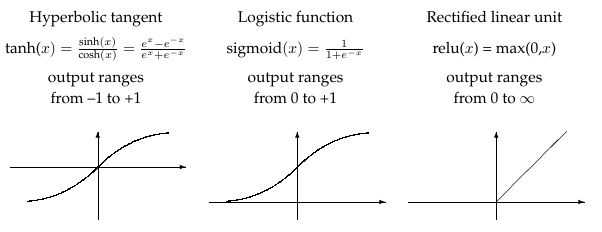
\includegraphics[width=0.9\textwidth]{activation_function.png}
\end{figure} 

A perceptron is the basic building blocks of neural network computation. Note that the output of a perceptron can be the input of another perceptron. 
In this manner, the perceptron can be interconnected to one and other, yielding complex networks. 

The following figure depicts a neural network with an additional layer between the input and output nodes:

\begin{figure}[h!]
\caption{A neural network with a hidden layer}
\centering
\begin{tikzpicture}[
plain/.style={
  draw=none,
  fill=none,
  },
net/.style={
  matrix of nodes,
  nodes={
    draw,
    circle,
    inner sep=10pt
    },
  nodes in empty cells,
  column sep=2cm,
  row sep=-9pt
  },
>=latex
]
\matrix[net] (mat)
{
|[plain]| \parbox{1.3cm}{\centering Input\\layer} & |[plain]| \parbox{1.3cm}{\centering Hidden\\layer} & |[plain]| \parbox{1.3cm}{\centering Output\\layer} \\
& |[plain]| \\
|[plain]| & \\
& |[plain]| \\
  |[plain]| & |[plain]| \\
& & \\
  |[plain]| & |[plain]| \\
& |[plain]| \\
  |[plain]| & \\
& |[plain]| \\    };
\foreach \ai [count=\mi ]in {2,4,...,10}
  \draw[<-] (mat-\ai-1) -- node[above] {Input \mi} +(-2cm,0);
\foreach \ai in {2,4,...,10}
{\foreach \aii in {3,6,9}
  \draw[->] (mat-\ai-1) -- (mat-\aii-2);
}
\foreach \ai in {3,6,9}
  \draw[->] (mat-\ai-2) -- (mat-6-3);
\draw[->] (mat-6-3) -- node[above] {Ouput} +(2cm,0);
\end{tikzpicture}

\rule{0in}{1.2em}$^\dag$\scriptsize For clarity, I don't show the bias nodes here.\\

\end{figure}    

This middle layer is called hidden layer. However, they are not really hidden; actually all the numerical values of each neuron in the hidden layer are all visible, but it is really hard to come up with a sensible interpretation on these numbers.  
When there are more than one hidden layers, the neural net is called deep neural net. However, the building blocks are still a simple perceptron. So, actually neural networks are simple and elegant computation operation\footnote{It seems to me that linking the perceptron is just like the simple Merge operation in the Minimalist Program.}; 
however, they extremely powerful. They are Turing-Complete machines \citep{siegelmann1991turing, graves2014neural}. \citet{siegelmann2003neural, siegelmann2012neural} even argues that neural networks are computations beyond the Turing limit. 

%\newpage
\subsection{Recurrent Neural Network}

Before we start to describe how a neural machine accomplishes the translation task, it is necessary to introduce a specific type of neural networks: Recurrent neural networks. 

Recall that the output of a perceptron can be the input of another perceptron. A interesting manipulation is to let the perceptron connect back to itself. With this manipulation, we have the Recurrent Neural Networks. As shown in the following figures, the hidden node is connected back to itself at each time step. As such, at each time step, there are two input sources of the hidden node: 1) the information from the past hidden node, and 2) the information from a new input node.       

\begin{figure}[h]
\caption{A recurrent neural network with a hidden layer. The hidden neuron ($h$) is connected to itself.}
\label{fig:rnn1}
\centering
\begin{tikzpicture}

  \node[neuron] (ht1) {$h$};
  \node[io,above=2em of ht1]  (yt1) {$y$};
  \node[io,below=2em of ht1]  (xt1) {$x$};
  \draw[conn] (ht1) -- (yt1);
  \draw[conn] (xt1) -- (ht1);
  \draw[thick,->,shorten >=1pt] (ht1.east) to [out=500,in=200,loop,looseness=4.8] (ht1.west);

\end{tikzpicture}
\end{figure}

\begin{figure}
\caption{A recurrent neural network with a hidden layer (unfolded depiction). This figure depicts exactly the same structure in figure \ref{fig:rnn1}, the hidden neuron $h_{t}$ is linked to its past $h_{t-1}$ and its future $h_{t+1}$. Here $t$ labels time step.}
\centering
\begin{tikzpicture}
\centering
  \node[neuron] (ht0)         {$h_{t-1}$};
  \node[io,above=2em of ht0] (yt)   {$y_{t-1}$};
  \node[io,below=2em of ht0] (xt)   {$x_{t-1}$};
  \draw[conn] (ht0) -- (yt);
  \draw[conn] (xt) -- (ht0);
  \node [left=of ht0] {\ldots};

  \node[neuron, right=of ht0] (ht1) {$h_{t}$};
  \node[io,above=2em of ht1]  (yt1) {$y_t$};
  \node[io,below=2em of ht1]  (xt1) {$x_t$};
  \draw[conn] (ht1) -- (yt1);
  \draw[conn] (xt1) -- (ht1);
  \draw [->] (ht0) -- (ht1);

  \node[neuron, right=of ht1] (ht2) {$h_{t+1}$};
  \node[io,above=2em of ht2]  (yt2) {$y_{t+1}$};
  \node[io,below=2em of ht2]  (xt2) {$x_{t+1}$};
  \draw[conn] (ht2) -- (yt2);
  \draw[conn] (xt2) -- (ht2);
  \draw [->] (ht1) -- (ht2);

  \node [right=of ht2] {\ldots};
\end{tikzpicture}
\end{figure}
\newpage
Is this manipulation useful? And if yes, why? It turns out Recurrent Neural Networks are really useful when we are interested in modeling a sequencing phenomenon and we believe that a fraction of the sequence will have an effect on the next coming fraction. The looping configuration opens the door to the history of the hidden neuron, and leads it to its future. 

Recurrent neural networks are widely used. Critically, the main theme of the dissertation, Neural Net Machine Translation, is also implemented with it. The coming section provides an overview of how neural networks translate languages. 

%\newpage
\section{Introduction to Neural Net Machine Translation}

My 3-year old daughter, Trina, is growing up in Tucson, Arizona, The languages that she encounters are English, Spanish and Mandarin Chinese, and thus she picks up English and Mandarin, and some Spanish. She is able to count the quantity of objects in the three languages. When I told her \textbf{in  Mandarin} that `we can bring two candies for Alice' on the way to her preschool, and she was able to tell her best friend, Alice, in her preschool that she will give her one candy \textbf{in English} (not two because Trina has to save one candy for herself).        

It is certain that a multilingual person can access the meaning of a sequence of strings in a language when he or she hears it, and then produces another sequence of strings in another different language with the same meaning. Given that a human brain is a neural network machine and artificial neural networks is similar to human neural networks, it fits our intuition that artificial neural networks can translate languages, of course. Actually, this is roughly how a neural net Machine Translation is implemented. Consider the following figure from \citet{luong17GitHub}.

\begin{figure}[h]
\caption{Encoder-decoder architecture - example of a general approach for NMT. An encoder converts a source sentence into a "meaning" vector which is passed through a decoder to produce a translation. (figure from \citet{luong17GitHub})}
\centering
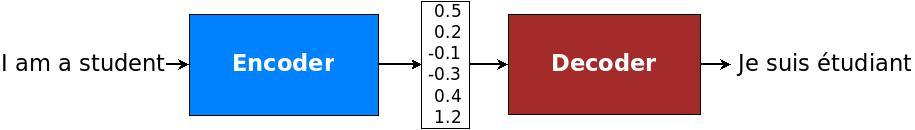
\includegraphics[width=0.9\textwidth]{encdec.jpg}
\end{figure} 

The figure outlines the heuristic of how neural networks computation may translate languages. When the neural net is fed with a source sentence, ``I am a student'', it will convert the sentence into a meaning representation or a thought vector. This is the encoding process. Based on this meaning representation, the machine then derives another sequence of words in the target language. This is the decoding process. Now we may take a close look of how the encoding and decoding process works. 

\subsection{Word Embedding}
The neural machine can only process numeral representations, so the first step is to convert words into numerical representations. Specifically each word will be represented as a vector. The central idea is to map each word onto a location in ``a meaning space'', and each vector is the geographical coordinates of the word. 
This process is called word embedding. The ideal word embedding system would have the properties that words with similar meanings will be neighbors in the meaning space. 
The most commonly used technique of building word embeddings is proposed in \citet{mikolov2013efficient, mikolov2013distributed}. Critically, this word embedding implementation follows the distributional semantics philosophy: the meaning of a word is defined by its distribution in a corpus. So, to build a word embedding model all we need is a corpus. The training data for Machine Translation is a parallel corpus, which gives us two corpora: the source language corpus and target language corpus. So, the training data is sufficient for building word embedding models\footnote{It is also a common practice to build the word embedding separately using a bigger corpus when the parallel corpus is too small.}. The following figure depicts how it is like when the word embeddings are mapped to a 2D space.   

\begin{figure}
\caption{Word Embeddings (figure from \citet{roweis2000nonlinear})}
\centering
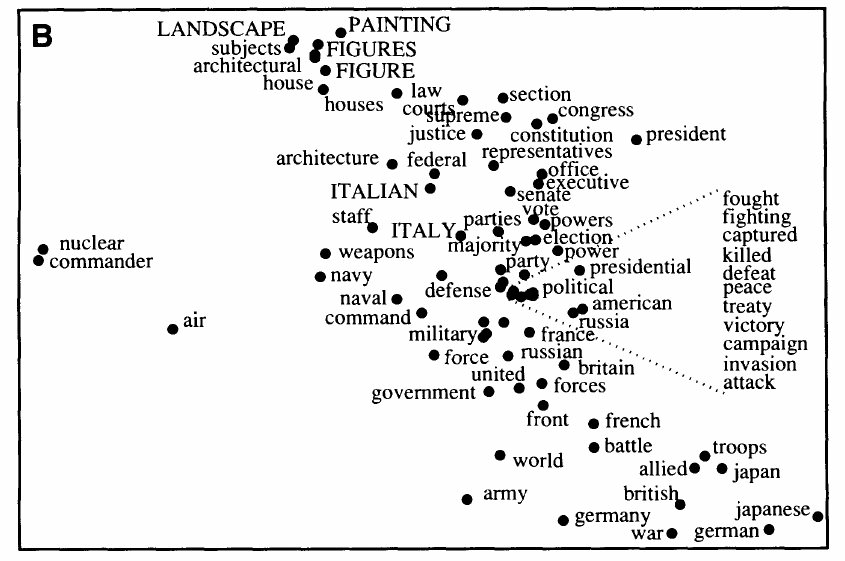
\includegraphics[width=0.9\textwidth]{word_emb.png}
\end{figure} 


\subsection{Encoding and Decoding}

A simple preprocessing on the data is to add tags that marks the boundaries of the sentences. Each word in the source sentence is sent to recurrent network machine incrementally. 
Note the looping configuration of recurrent neural networks makes it possible for the machine to accumulate the information of all the words. When the tag that marks the end of the source sentence is fed into the machine, the encoding process is completed, and the value of the hidden neurons at this time is the meaning representation of the source sentence.  

Given the meaning representation, now the machine starts to decode. At each time step, it emits a word in the target language. The emitted word in the target language is copied and served as input in the next time step of decoding. So that the output sentence can have the context information of the previous word; this trick ensures the fluency of the output sentence. 

Consider the following figure from \citet{luong17GitHub} for a concrete example of how the encoding-decoding process works.  

\begin{figure}[h]
\caption{Neural Machine Translation (figure from \citet{luong17GitHub}).}
\centering
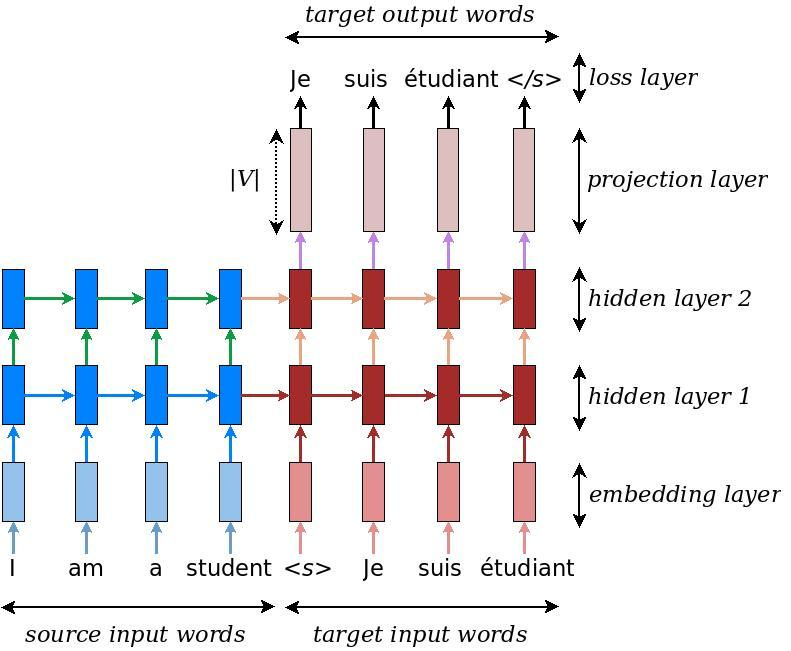
\includegraphics[width=0.9\textwidth]{seq2seq.jpg}
\end{figure} 

In the current example, we are trying to translate a source sentence ``I am a student'' into a target sentence ``Je suis \'{e}tudiant''. Here, ``<s>'' marks the end of the source sentences and the starting point of the decoding process. 
So, at the time step of  ``<s>'', the vector in the hidden neurons is the meaning representation. In the decoding process, the first emitted word is ``Je''. Note that ``Je'' is sent back as the input in the next time step, when ``suis'' is emitted. Now we may pay attention to what the given information is when the machine is emitting ``suis''. Specifically, the given information is: 1) thought vectors plus ``je'' in the hidden layers, and 2) ``je'' from the input node. When the machine emitted the tag, ``</s>'', the decoding process is completed. 

This section covers the basic structure of a neural Machine Translation system proposed in \citet{cho2014properties, cho2014learning}.  


\subsection{Adding Attention Mechanism}

The meaning vector is the accumulated information of all the bits in the source sentence. The decoding process needs to sort out all the bits from the mixed information in the meaning vector. Actually, this is a lot to ask. The task is like to figure out what ingredients are from a pot of hot and sour soup by tasting the soup. To facilitate the sorting task of the decoding processing, \citet{bahdanau2014neural} and \citet{luong2015effective} propose methods to direct the decoder's attention to the relevant bits in the source sentence. Take the soup analogy again. With the attention mechanism, to guess what the ingredient is, the given information is now the taste of vinegar, in addition to the taste of the mixed-up soup in this time step. So that the chance of getting the right answer (i.e. vinegar) is much higher. And in the next time step, in addition to the taste of the mixed-up soup, one is also given the taste of pepper, and so on.   

The following figure from \citet{luong17GitHub} nicely depicts how the attention mechanism works. 

\begin{figure}[h]
\caption{Attention mechanism - example of an attention-based NMT system as described in \citet{luong2015effective} (figure from \citet{luong17GitHub})}
\centering
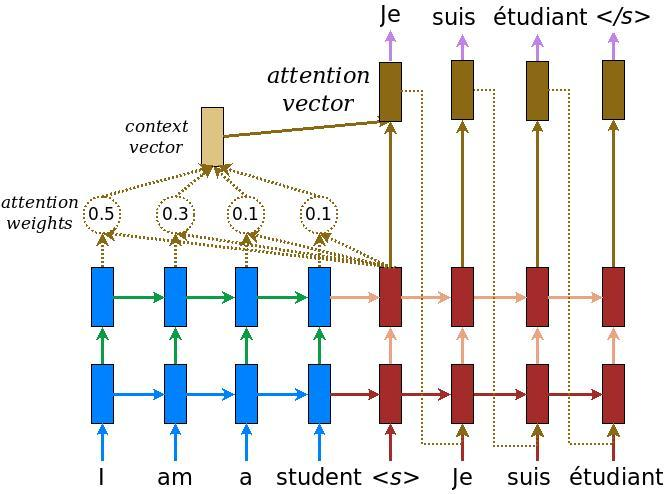
\includegraphics[width=0.9\textwidth]{attention_mechanism.jpg}
\end{figure} 

In the figure, the task is to translate a source sentence ``I am a student'' into a target sentence ``Je suis \'{e}tudiant''.
The encoding process is the same, but in the decoding process additional information is also provide. In the current example, when the decoder emits the word ``je'', it is given the meaning vector, and additionally the attention mechanism also gives the decoder 50\% of the information of ``I'', 30\% of the information of ``am'', 10\% of the information of ``a'', and 10\% of the information of ``student''. In this manner, the machine's attention is directed to ``I'' when the supposed emitted word is ``Je''. The attention mechanism is very similar to alignment; in the current example, ``Je'' is 50\% aligned to ``I'', 30\% aligned to ``am'', 10\% aligned to ``a'', and 10\% aligned to ``student''. 

\subsection{Summary of Neural Net Machine Translation: interlingua plus string alignment}

The state-of-the-art neural network Machine Translation is the combination of the encoding-decoding algorithm and the attention algorithm. The meaning vector in the encoding-decoding algorithm actually can be viewed as the holy grail in translation, the interlingua representation. The attention algorithm is a reminiscence of the string alignment approach used in statistical Machine Translation. So, neural net Machine Translation is actually a combination of interlingua  translation approach and string alignment approach.   


\section{A Quick Historical Overview of Machine Translation and Conclusion}

Machine Translation is to automate the process of translating one natural language to another using computers. The first peak of the developments of Machine Translation started in the 1940s but terminated in 1966. During this period of time, with the advent of the first computers, researchers held high expectations in Machine Translation and lots of resources are shifted into this area. 
However, in 1966 a report of the Automatic Language Processing Advisory Committee \citep{pierce1966language} terminated this `Machine Translation rush' as it revealed that too many funds and resources were shifted to Machine Translation without yielding proportional scientific developments. 
In 1990s, with the advent of Statistical Machine Translation approach developed at IBM, the Machine Translation came back as one of popular scientific areas. 
Now with the advent of the technique of Artificial Neural Net Machine Learning and other natural language processing techniques, Machine Translation is one of the most dynamic research areas.    
